\documentclass[11pt]{article}

% -----------------------------------------------------------------------------
% Typography and page design
% -----------------------------------------------------------------------------
\usepackage[a4paper,margin=2.15cm,headheight=22pt]{geometry}
\usepackage[T1]{fontenc}
\usepackage{lmodern}
\usepackage{microtype}
\usepackage{xcolor}
\usepackage{amsmath,amssymb,mathtools}
\usepackage{booktabs,tabularx,array}
\usepackage{enumitem}
\usepackage{titlesec}
\usepackage{fancyhdr}
\usepackage{tikz}
\usepackage[most]{tcolorbox}
\usepackage[hidelinks]{hyperref}
\usetikzlibrary{arrows.meta,positioning,calc,fit}

% Restrained black-and-white palette for print and screen.
\definecolor{navy}{gray}{0.05}
\definecolor{blue}{gray}{0.05}
\definecolor{paleBlue}{gray}{0.96}
\definecolor{paleGold}{gray}{0.96}
\definecolor{gold}{gray}{0.30}
\definecolor{ink}{gray}{0.05}
\definecolor{muted}{gray}{0.35}
\definecolor{rulegray}{gray}{0.72}

\color{ink}
\setlength{\parindent}{0pt}
\setlength{\parskip}{0.55em}
\setlist[itemize]{leftmargin=1.5em,itemsep=0.18em,topsep=0.25em}
\setlist[enumerate]{leftmargin=1.65em,itemsep=0.2em,topsep=0.3em}
\renewcommand{\arraystretch}{1.18}

\titleformat{\section}
  {\Large\bfseries\color{navy}}{\thesection}{0.65em}{}
\titleformat{\subsection}
  {\large\bfseries\color{blue}}{\thesubsection}{0.55em}{}
\titlespacing*{\section}{0pt}{1.45em}{0.55em}
\titlespacing*{\subsection}{0pt}{1.0em}{0.35em}

\pagestyle{fancy}
\fancyhf{}
\lhead{\small\color{muted}Assignment 2}
\rhead{\small\color{muted}Vector Embedding for Capability Composition}
\cfoot{\small\color{muted}\thepage}
\renewcommand{\headrulewidth}{0.35pt}
\renewcommand{\headrule}{\hbox to\headwidth{\color{rulegray}\leaders\hrule height \headrulewidth\hfill}}

% -----------------------------------------------------------------------------
% Reusable components
% -----------------------------------------------------------------------------
\newtcolorbox{keybox}[1][]{
  enhanced,
  sharp corners,
  colback=black!5,
  colframe=black!5,
  colbacktitle=black!13,
  coltitle=black,
  fonttitle=\bfseries\large,
  boxrule=0pt,
  left=12pt,right=12pt,top=10pt,bottom=10pt,
  lefttitle=12pt,righttitle=12pt,toptitle=6pt,bottomtitle=6pt,
  before skip=10pt,after skip=10pt,
  #1
}

\newtcolorbox{warningbox}[1][]{
  enhanced,
  sharp corners,
  colback=black!5,
  colframe=black!5,
  colbacktitle=black!13,
  coltitle=black,
  fonttitle=\bfseries\large,
  boxrule=0pt,
  left=12pt,right=12pt,top=10pt,bottom=10pt,
  lefttitle=12pt,righttitle=12pt,toptitle=6pt,bottomtitle=6pt,
  before skip=10pt,after skip=10pt,
  #1
}

\newtcolorbox{examplebox}[1]{
  enhanced,
  sharp corners,
  colback=black!4,
  colframe=black!4,
  colbacktitle=black!12,
  coltitle=black,
  title={#1},
  fonttitle=\bfseries\large,
  boxrule=0pt,
  left=12pt,right=12pt,top=10pt,bottom=10pt,
  lefttitle=12pt,righttitle=12pt,toptitle=6pt,bottomtitle=6pt,
  before skip=10pt,after skip=10pt
}

\newcommand{\term}[1]{\textbf{\color{navy}#1}}
\newcommand{\code}[1]{\texttt{#1}}
\newcommand{\R}{\mathbb{R}}
\newcommand{\true}{\texttt{true}}
\newcommand{\false}{\texttt{false}}

\newcolumntype{L}[1]{>{\raggedright\arraybackslash}p{#1}}
\newcolumntype{Y}{>{\raggedright\arraybackslash}X}

% -----------------------------------------------------------------------------
% Motivation diagrams
% -----------------------------------------------------------------------------
\newcommand{\relationshipdiagram}[5]{%
\begin{tikzpicture}[x=0.86cm,y=0.86cm,>=Latex]
  \draw[->,thick] (0,0) -- (0,3.25);
  \draw[->,thick] (0,0) -- (3.65,0);
  \draw[->,thick] (0,0) -- (-1.65,-1.05);
  \node[font=\small,align=center] at (1.85,-0.72) {#5};
  \node[draw=black!65,fill=black!7,rounded corners=1pt,
        minimum width=1.15cm,minimum height=.52cm,font=\small,align=center]
        (a) at (0.75,2.6) {#1};
  \node[draw=black!65,fill=black!7,rounded corners=1pt,
        minimum width=1.15cm,minimum height=.52cm,font=\small,align=center]
        (b) at (0.75,1.15) {#2};
  \node[draw=black!65,fill=white,rounded corners=1pt,
        minimum width=1.05cm,minimum height=.52cm,font=\small,align=center]
        (c) at (2.65,2.6) {#3};
  \node[draw=black!65,fill=white,rounded corners=1pt,
        minimum width=1.05cm,minimum height=.52cm,font=\small,align=center]
        (d) at (2.65,1.15) {#4};
  \draw[->,dashed,black!60,thick] (a.east) -- (c.west);
  \draw[->,dashed,black!60,thick] (b.east) -- (d.west);
\end{tikzpicture}%
}

\newcommand{\capabilitydiagram}{%
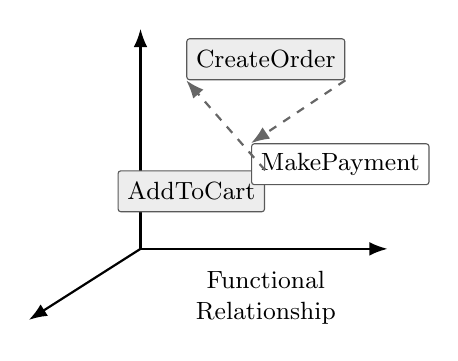
\begin{tikzpicture}[x=0.86cm,y=0.86cm,>=Latex]
  \draw[->,thick] (0,0) -- (0,3.25);
  \draw[->,thick] (0,0) -- (3.65,0);
  \draw[->,thick] (0,0) -- (-1.65,-1.05);
  \node[font=\small,align=center] at (1.85,-0.72) {Functional\\Relationship};
  \node[draw=black!65,fill=black!7,rounded corners=1pt,
        minimum width=1.3cm,minimum height=.52cm,font=\small,align=center]
        (createorder) at (1.85,2.8) {CreateOrder};
  \node[draw=black!65,fill=black!7,rounded corners=1pt,
        minimum width=1.15cm,minimum height=.52cm,font=\small,align=center]
        (addtocart) at (0.75,0.85) {AddToCart};
  \node[draw=black!65,fill=white,rounded corners=1pt,
        minimum width=1.25cm,minimum height=.52cm,font=\small,align=center]
        (makepayment) at (2.95,1.25) {MakePayment};
  \draw[->,dashed,black!60,thick]
        (addtocart.north east) -- (createorder.south west);
  \draw[->,dashed,black!60,thick]
        (createorder.south east) -- (makepayment.north west);
\end{tikzpicture}%
}

\begin{document}
\thispagestyle{plain}

% -----------------------------------------------------------------------------
% Title
% -----------------------------------------------------------------------------
\begin{center}
  {\bfseries\large ASSIGNMENT 2}\par
  \vspace{0.3em}
  {\color{navy}\bfseries\LARGE Design of a Vector Embedding\par}
  \vspace{0.12em}
  {\color{navy}\bfseries\LARGE for Capability Composition}\par
  \vspace{0.65em}
  {\color{muted}\large Formal representations, compatibility, and compositional reasoning}
\end{center}

\section{Motivation}

In 2013, a team of researchers at Google including, \textbf{Tomáš Mikolov,
Kai Chen, Greg Corrado, Ilya Sutskever, and Jeff Dean}, introduced Word2Vec and helped move
modern natural-language processing from symbolic representations of words toward
distributed vector representations. Word2Vec places words in a continuous vector space so
that useful semantic relationships are preserved. Words with similar meanings or patterns
of use lie close to one another, while algebraic relationships in the space can encode
meaningful analogies.

\begin{center}
\begin{minipage}[t]{0.46\textwidth}
\centering
{\bfseries Word2Vec: Semantic relationships\\between words}\par
\vspace{0.15cm}
\relationshipdiagram{Woman}{Queen}{Man}{King}{Semantic\\Relationship}
\end{minipage}
\hfill
\begin{minipage}[t]{0.46\textwidth}
\centering
{\bfseries This Assignment: Functional relationships\\between capabilities}\par
\vspace{0.15cm}
\capabilitydiagram
\end{minipage}
\end{center}

While Word2Vec captures \emph{semantic} relationships between words, this assignment
focuses on \emph{functional} relationships between capabilities in an application domain.
Instead of meaning, the concern is which capabilities can work together, what they require,
what they produce, and how they transform the state of a system.

\begin{keybox}[title={Definition: Capability}]
A \textbf{capability} is a well-defined, reusable operation or service that performs a
specific function within a system. It is characterized formally by what it requires
(inputs, preconditions, and resources), what it does (effects), what it produces (outputs),
and the constraints and quality attributes under which it operates.
\end{keybox}

\begin{keybox}[title={Central task}]
Design, implement, and evaluate a problem-specific vector
representation for formally specified states, goals, and executable capabilities. The
representation should preserve the functional relationships required to identify compatible
capabilities and construct complex capabilities from simpler ones.
\end{keybox}

\clearpage
\section{Objective and Scope}

In Assignment 1, you developed a planning and orchestration mechanism that searches for a
sequence of transitions capable of transforming an initial state into a goal state while
respecting constraints. This assignment changes the focus from \emph{finding the sequence}
to \emph{representing the operations that make up the sequence}. These operations are called
\term{capabilities}.

Your embedding should investigate relationships among:

\begin{center}
\begin{tabularx}{0.94\textwidth}{@{}YYYY@{}}
states & goals & capabilities & preconditions \\
effects & inputs and outputs & constraints & resources \\
cost & reliability & availability & capability composition
\end{tabularx}
\end{center}

The ultimate objective is to represent complex capabilities as compositions of smaller
capabilities.

\begin{warningbox}[title={Important scope boundary}]
You are \emph{not} required to redesign or improve the
LPA*/D* Lite planner from Assignment 1. BFS, DFS, A*, D* Lite, LPA*, path search, and
replanning algorithms are outside the scope of this assignment. The planner is background
context only.
\end{warningbox}

\subsection{Relationship to Assignment 1}

In Assignment 1, states and transitions were used to find a sequence of actions that
transforms an initial state into a goal state. In this assignment, the focus changes from
\emph{finding the sequence} to \emph{representing the operations that make up the
sequence}.

\begin{center}
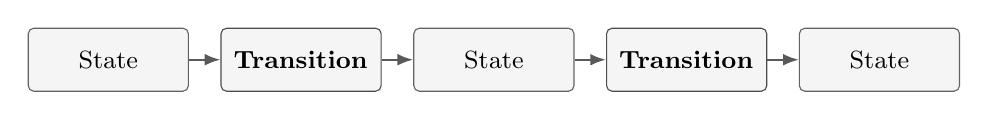
\begin{tikzpicture}[
  node distance=4mm,
  state/.style={draw=blue!65,fill=paleBlue,rounded corners=2pt,minimum height=8mm,
                text width=18mm,align=center,font=\small},
  trans/.style={draw=gold,fill=paleGold,rounded corners=2pt,minimum height=8mm,
              text width=18mm,align=center,font=\small\bfseries},
  arr/.style={-{Latex[length=2mm]},thick,color=muted}
]
\node[state] (s0) {State};
\node[trans,right=of s0] (t0) {Transition};
\node[state,right=of t0] (s1) {State};
\node[trans,right=of s1] (t1) {Transition};
\node[state,right=of t1] (s2) {State};
\draw[arr] (s0)--(t0);
\draw[arr] (t0)--(s1);
\draw[arr] (s1)--(t1);
\draw[arr] (t1)--(s2);
\end{tikzpicture}\par
{\small\color{muted}Assignment 1: a sequence of transitions between states}
\end{center}

\begin{center}
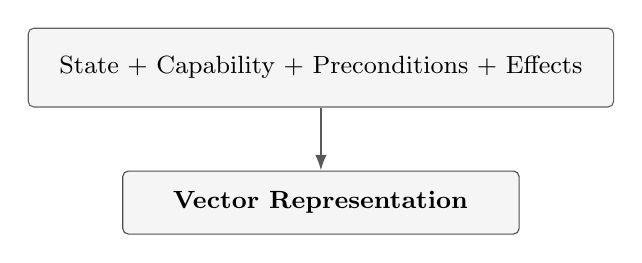
\begin{tikzpicture}[
  node distance=4mm,
  block/.style={draw=blue!65,fill=paleBlue,rounded corners=2pt,minimum height=10mm,
                text width=72mm,align=center,font=\small},
  vec/.style={draw=gold,fill=paleGold,rounded corners=2pt,minimum height=8mm,
              text width=48mm,align=center,font=\small\bfseries},
  arr/.style={-{Latex[length=2mm]},thick,color=muted}
]
\node[block] (comp) {State + Capability + Preconditions + Effects};
\node[vec,below=8mm of comp] (vecrep) {Vector Representation};
\draw[arr] (comp)--(vecrep);
\end{tikzpicture}\par
{\small\color{muted}Assignment 2: representing the operation itself}
\end{center}

A transition in Assignment 1 can be viewed conceptually as an operation performed on a
state. In Assignment 2, these operations are represented as capabilities. The
planning/replanning algorithm from Assignment 1 remains outside the scope of this
assignment; it is background context only.

\section{Formal Application Model}

A real-world application is represented formally as follows.

\begin{keybox}[title={Formal application model}]
\[
  \mathcal{A}=(\mathcal{S},\mathcal{C},S_I,G,\mathcal{R},\mathcal{K})
\]
\begin{tabularx}{\textwidth}{@{}L{1.4cm}Y@{}}
\(\mathcal{S}\) & State space of the application \\[0.3em]
\(\mathcal{C}\) & Set of available capabilities \\[0.3em]
\(S_I\) & Initial state \\[0.3em]
\(G\) & Goal specification \\[0.3em]
\(\mathcal{R}\) & Set of available resources \\[0.3em]
\(\mathcal{K}\) & Global constraints and policies
\end{tabularx}
\end{keybox}

The initial state, goal, and capabilities are provided in formal rather than
natural-language representations.

\subsection{States and the initial state}

A \term{state} describes the condition of the application at a particular point in time:
\[
  S=\{(x_1,v_1),(x_2,v_2),\ldots,(x_n,v_n)\},
\]
where \(x_i\) is a state variable and \(v_i\) is its current value. Variables may be
Boolean, integer, real-valued, categorical, enumerated, or structured. The initial state
\(S_I\in\mathcal{S}\) specifies the condition before execution begins.

\begin{keybox}[title={Example initial state}]
\begin{tabularx}{\textwidth}{@{}lY@{}}
\code{User.authenticated} & \code{true} \\[0.3em]
\code{User.role} & \code{CUSTOMER} \\[0.3em]
\code{Cart.exists} & \code{true} \\[0.3em]
\code{Cart.item\_count} & \code{3} \\[0.3em]
\code{Order.exists} & \code{false} \\[0.3em]
\code{Payment.status} & \code{NOT\_STARTED} \\[0.3em]
\code{Inventory.available} & \code{true} \\[0.3em]
\code{Notification.sent} & \code{false}
\end{tabularx}
\end{keybox}

\subsection{Goal specification}

A goal is a set of desired conditions,
\[
  G=\{g_1,g_2,\ldots,g_m\}.
\]
A state \(S\) satisfies the goal when \(S\models G\).

\begin{examplebox}{Example goal specification}
\begin{tabularx}{\textwidth}{@{}Yc@{}}
\code{Order.exists} & \code{true} \\[0.45em]
\code{Payment.status} & \code{SUCCESS} \\[0.45em]
\code{Notification.sent} & \code{true}
\end{tabularx}
\end{examplebox}
The overall application seeks a transformation
\[
  S_I \longrightarrow S_1 \longrightarrow \cdots \longrightarrow S_n
  \qquad\text{such that}\qquad S_n\models G.
\]
Finding this sequence is a planning task and is not part of this assignment.

\section{Formal Capability Model}

A \term{capability} is a well-defined, reusable operation or service that performs a
specific function within a system. It transforms application state and is characterized by
what it requires, what it produces, how it changes the state, and the conditions under
which it operates.

\begin{keybox}[title={Formal capability representation}]
\[
  C_i=(T_i,I_i,O_i,P_i,E_i,K_i,R_i,Q_i,\operatorname{Rel}_i,A_i,M_i)
\]
\small
\begin{tabularx}{\textwidth}{@{}L{2.2cm}Y@{}}
\toprule
\textbf{Component} & \textbf{Meaning} \\
\midrule
\(T_i\) & Capability type \\[0.25em]
\(I_i, O_i\) & Input and output specifications \\[0.25em]
\(P_i, E_i\) & Preconditions and effects \\[0.25em]
\(K_i\) & Capability-specific constraints \\[0.25em]
\(R_i\) & Resource requirements \\[0.25em]
\(Q_i\) & Cost and other quality attributes \\[0.25em]
\(\operatorname{Rel}_i\) & Reliability \\[0.25em]
\(A_i\) & Availability \\[0.25em]
\(M_i\) & Execution mechanism \\
\bottomrule
\end{tabularx}
\end{keybox}

This structure should contain enough information to reason about a capability without
requiring a natural-language description.

\subsection{Capability type and execution mechanism}

The type identifies the broad mechanism through which a capability is realized:
\[
T_i\in\{\code{API},\code{DATABASE},\code{GUI},\code{EVENT},\code{FUNCTION},
\code{FILE},\code{COMPUTATION},\code{MESSAGE},\code{SERVICE}\}.
\]
The execution mechanism \(M_i\) records implementation-specific details.

\begin{examplebox}{Examples of execution mechanisms}
\small
\begin{tabularx}{\textwidth}{@{}L{2.2cm}Y@{}}
\toprule
\textbf{Type} & \textbf{Example mechanism} \\
\midrule
API & \code{method = POST}\\ & \code{endpoint = /orders} \\[0.45em]
Database & \code{operation = INSERT}\\ & \code{table = orders} \\[0.45em]
GUI & \code{action = CLICK}\\ & \code{component = submit\_button} \\[0.45em]
Event & \code{trigger = OrderCreated}\\ & \code{handler = SendNotification} \\
\bottomrule
\end{tabularx}
\end{examplebox}

Your design should determine how strongly type and mechanism should influence the
embedding, and whether implementation-specific information belongs in the main vector or
in a separate representation.

\subsection{Inputs and outputs}

A capability may require inputs and produce outputs.

\begin{examplebox}{Input specification}
\[
 I_i=\{i_1,\ldots,i_p\}
\]
Each input is described separately:
\[
 i_j=(\text{name},\text{type},\text{domain},\text{required}).
\]
\textbf{Example}
\[
i=(\code{cart\_id},\code{UUID},\text{valid UUIDs},\true).
\]
\end{examplebox}

\begin{examplebox}{Output specification}
\[
 O_i=\{o_1,\ldots,o_q\}
\]
Each output is described separately:
\[
 o_j=(\text{name},\text{type},\text{domain}).
\]
\textbf{Example}
\[
o=(\code{order\_id},\code{UUID},\text{valid UUIDs}).
\]
\end{examplebox}

For \code{CreateOrder}, the examples above represent a required input and a produced
output. If an output \(o\in O_i\)
satisfies an input requirement \(i\in I_j\), then \(C_i\) may provide data required by
\(C_j\).

\subsection{Preconditions and effects}

The precondition set \(P_i=\{p_1,\ldots,p_r\}\) describes when a capability may run:
\[
  C_i\text{ is applicable to }S \quad\Longleftrightarrow\quad S\models P_i.
\]

\begin{examplebox}{Example preconditions}
\begin{itemize}[itemsep=0.45em]
\item \code{authenticated = true}
\item \code{customer\_exists = true}
\item \code{cart\_exists = true}
\item \code{cart\_item\_count > 0}
\item \code{inventory\_available = true}
\end{itemize}
\end{examplebox}

The effect set \(E_i=\{e_1,\ldots,e_s\}\) specifies the resulting state changes. If
\(C_i\) is applicable, then
\[
  C_i:S\longrightarrow S',\qquad S'=\operatorname{Apply}(S,E_i).
\]
\begin{examplebox}{Example effects}
\begin{itemize}[itemsep=0.45em]
\item \code{Order.exists = true}
\item \code{Order.status = CREATED}
\item \code{Cart.locked = true}
\end{itemize}
\end{examplebox}

\begin{keybox}[title={Example capability: CreateOrder}]
\begin{tabularx}{\textwidth}{@{}L{2.7cm}Y@{}}
\textbf{Preconditions} & \code{CartExists = true}\\
& \code{CartItemCount > 0} \\[0.65em]
\textbf{Effects} & \code{OrderExists = true}\\
& \code{OrderStatus = CREATED}
\end{tabularx}
\[
  \text{State }S \xrightarrow{\;\code{CreateOrder}\;} \text{State }S'.
\]
\end{keybox}

\subsection{Constraints and resources}

Capability-specific constraints are represented as \(K_i=\{k_1,\ldots,k_t\}\). They
may include input, state, resource, security, temporal, dependency, and domain-specific
restrictions.

\begin{examplebox}{Example constraints}
\begin{itemize}[itemsep=0.5em]
\item \code{quantity > 0}
\item \code{quantity <= inventory\_available}
\item \code{payment\_amount <= transaction\_limit}
\item \code{user.role in \{CUSTOMER, ADMIN\}}
\end{itemize}
\end{examplebox}

Resource requirements are represented as \(R_i=\{r_1,\ldots,r_u\}\).

\begin{examplebox}{Example resource requirements}
\begin{tabularx}{\textwidth}{@{}YY@{}}
\textbullet\ Database & \textbullet\ Authentication token \\[0.45em]
\textbullet\ Payment gateway & \textbullet\ Network \\[0.45em]
\textbullet\ File system & \textbullet\ GPU \\[0.45em]
\textbullet\ External service &
\end{tabularx}
\end{examplebox}

Resource requirements must be considered in the capability representation.

\subsection{Cost}

A capability may have several operational costs or quality attributes:
\[
  Q_i=(C_{\mathrm{time}},C_{\mathrm{resource}},C_{\mathrm{money}},
       C_{\mathrm{risk}},C_{\mathrm{energy}}).
\]
\begin{examplebox}{Illustrative operational attributes}
\begin{tabularx}{\textwidth}{@{}Yc@{}}
Execution time & \code{100 ms} \\[0.45em]
Monetary cost & \code{0.01} \\[0.45em]
Resource cost & \code{2} \\[0.45em]
Risk & \code{0.1}
\end{tabularx}
\end{examplebox}

You may introduce additional quality attributes where appropriate.

\subsection{Reliability and Availability}

\textbf{Reliability.} The reliability of a capability represents its probability of
success:
\[
  \operatorname{Rel}_i\in[0,1].
\]
For example, \(\operatorname{Rel}_i=0.99\) represents an approximate success probability
of 0.99 under the specified conditions. The embedding design should investigate whether
reliability should be represented explicitly, indirectly, or separately from the semantic
representation.

\textbf{Availability.} A capability may be available or unavailable at a particular point
in time. A simple representation is
\[
  A_i\in\{0,1\}.
\]
For dynamic systems, availability may instead be represented as
\[
  A_i(t)\in\{0,1\}.
\]
For example, an external service may be available only during a specified period. The
embedding design should investigate whether these operational properties should be embedded
directly, represented separately, or handled through a combination of approaches.

\section{Capability Composition}

Consider two capabilities
\[
  C_1:S_0\rightarrow S_1,\qquad C_2:S_1\rightarrow S_2.
\]
If the outputs and effects of \(C_1\) satisfy the inputs and preconditions of \(C_2\), then
\(C_2\circ C_1\) is a valid composition. The resulting complex capability is
\[
  C_{12}=C_2\circ C_1:S_0\rightarrow S_2.
\]
Composition may be extended recursively, for example
\(C_{123}=C_3\circ C_2\circ C_1\). A central objective is to determine how such
compositions should be represented in the proposed vector space.

\begin{center}
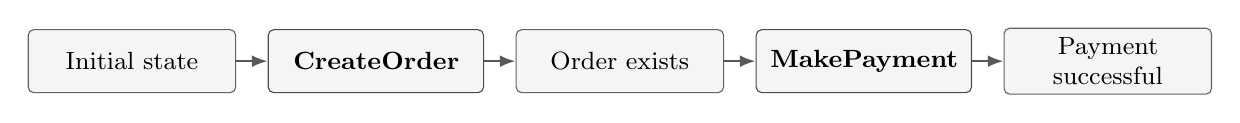
\begin{tikzpicture}[
  node distance=4mm,
  state/.style={draw=blue!65,fill=paleBlue,rounded corners=2pt,minimum height=8mm,
                text width=24mm,align=center,font=\small},
  capability/.style={draw=gold,fill=paleGold,rounded corners=2pt,minimum height=8mm,
              text width=25mm,align=center,font=\small\bfseries},
  arr/.style={-{Latex[length=2mm]},thick,color=muted}
]
\node[state] (s0) {Initial state};
\node[capability,right=of s0] (c1) {CreateOrder};
\node[state,right=of c1] (s1) {Order exists};
\node[capability,right=of s1] (c2) {MakePayment};
\node[state,right=of c2] (s2) {Payment successful};
\draw[arr] (s0)--(c1);
\draw[arr] (c1)--(s1);
\draw[arr] (s1)--(c2);
\draw[arr] (c2)--(s2);
\end{tikzpicture}
\end{center}

\begin{examplebox}{Composite capability: CompletePurchase}
\code{CreateOrder} produces the effect
\(\code{OrderExists}=\true\).

This satisfies a precondition of \code{MakePayment}, which then produces
\(\code{PaymentStatus}=\code{SUCCESS}\). Therefore,
\[
  \code{CompletePurchase}=\code{MakePayment}\circ\code{CreateOrder}.
\]
\end{examplebox}

\section{Embedding Design Problem}

Given \(\mathcal{P}=(\mathcal{S},G,\mathcal{C})\), design embeddings for the formal
entities. You may use separate representations,
\[
  \phi_S:\mathcal{S}\rightarrow\R^{d_s},\qquad
  \phi_G:G\rightarrow\R^{d_g},\qquad
  \phi_C:\mathcal{C}\rightarrow\R^{d_c},
\]
or a unified representation \(\phi:(\mathcal{S},G,\mathcal{C})\rightarrow\R^d\). The
choice is part of the assignment.

An embedding converts a formal entity into a numerical vector, for example
\[
 \text{formal capability}\xrightarrow{\ \phi_C\ }
 [0.21,-0.43,0.71,\ldots,0.18].
\]
Its purpose is not merely to assign a unique number. It should preserve useful
relationships among capabilities, states, and goals.

\subsection{Required properties}

Your design must investigate the following properties.

\begin{enumerate}[label=\textbf{\arabic*.}]
  \item \term{Capability identity.} Functionally different capabilities should be
  distinguishable.

  \item \term{State awareness.} The representation should capture the relationship between
  a capability and the states on which it operates.

  \item \term{Precondition--effect compatibility.} It should capture relationships such as
  \(E_i\Rightarrow P_j\), which may permit \(C_i\rightarrow C_j\).

  \item \term{Input--output compatibility.} It should represent cases where one
  capability's output satisfies another capability's input requirements.

  \item \term{Similarity and composability.} Functional resemblance and composability are
  not the same. Similar capabilities need not compose; composition requires compatible
  outputs/effects and inputs/preconditions. For example,
  \code{CreateOrder -> MakePayment} is compatible, whereas
  \code{CreateOrder -> SendNotification} is not necessarily compatible. Explain how
  similarity is used when evaluating capability relationships.

  \item \term{Composition.} Provide a meaningful representation for \(C_i\circ C_j\) and,
  where appropriate, \(C_1\circ C_2\circ\cdots\circ C_n\).

  \item \term{Goal relevance.} Allow the relationship between capabilities and the desired
  goal to be investigated.

  \item \term{Operational properties.} Determine how cost, reliability, availability,
  constraints, and resources should be embedded or represented separately.
\end{enumerate}

\clearpage
\begin{keybox}[title={No prescribed embedding technique}]
Study relevant representation and embedding methods;
analyse their strengths and limitations; then design, justify, implement, and evaluate a
solution specifically for capability composition. You may adapt or combine existing ideas,
but merely applying an existing embedding model is not sufficient.
\end{keybox}

\section{Required Experiments}

Construct experiments using formally specified application problems.

\begin{enumerate}[label=\textbf{\arabic*.},leftmargin=2em,itemsep=1.3em,topsep=0.7em]

\item \textbf{Capability compatibility.}

Given \(C_1,C_2,C_3\), where \(C_1\) composes with \(C_2\) but not \(C_3\), investigate
whether the representation distinguishes the relationships. Use the following pattern:

\begin{center}
\small
\renewcommand{\arraystretch}{1.25}
\begin{tabularx}{\linewidth}{@{}L{3.1cm}L{5.0cm}Y@{}}
\toprule
\textbf{Capability} & \textbf{Precondition} & \textbf{Effect} \\
\midrule
\(C_1\): CreateOrder & No additional precondition & \code{OrderExists = true} \\[0.55em]
\(C_2\): MakePayment & \code{OrderExists = true} & --- \\[0.55em]
\(C_3\): CancelCart & \code{OrderExists = false} & --- \\
\bottomrule
\end{tabularx}
\renewcommand{\arraystretch}{1.18}
\end{center}

Therefore, \(C_1\rightarrow C_2\) is compatible and
\(C_1\rightarrow C_3\) is incompatible.

\item \textbf{Capability composition.}

Given \(C_1\rightarrow C_2\rightarrow C_3\), construct the composite capability and
investigate how its vector relates to the vectors of \(C_1,C_2,C_3\).

\item \textbf{Alternative implementations.}

Provide capabilities that produce similar effects through different mechanisms, such as an
API, database, and GUI.

Test whether the embedding captures their functional relationship without incorrectly
treating their implementations as identical.

\item \textbf{Irrelevant capabilities.}

Introduce capabilities that do not contribute to the specified goal. Test whether the
representation distinguishes useful capabilities from irrelevant ones.

\item \textbf{Operational attributes.}

Investigate the influence of at least two of the following: cost, reliability, availability,
risk, and resource requirement.

\end{enumerate}

\clearpage
\section{Evaluation Criteria}

Evaluate the proposed embedding against every question below.

\begin{center}
\small
\renewcommand{\arraystretch}{1.3}
\begin{tabularx}{\textwidth}{@{}L{4.5cm}Y@{}}
\toprule
\textbf{Property} & \textbf{Question to be evaluated} \\
\midrule
Capability representation & Can different capabilities be represented distinctly? \\[0.35em]
State relationship & Does the representation capture the relationship between capabilities
and states? \\[0.35em]
Precondition--effect compatibility & Can composable capabilities be distinguished from
incompatible ones? \\[0.35em]
Input--output compatibility & Can dependencies between capabilities be represented? \\[0.35em]
Composition & Can complex capabilities be represented from smaller capabilities? \\[0.35em]
Goal relevance & Can the relationship between capabilities and goals be identified? \\[0.35em]
Operational properties & Can cost, reliability, availability, and constraints be represented
appropriately? \\[0.35em]
Consistency & Does the representation behave consistently across different problems? \\[0.35em]
Efficiency & What are the computational and storage requirements? \\
\bottomrule
\end{tabularx}
\renewcommand{\arraystretch}{1.18}
\end{center}

\section{Deliverables}

Submit all four components below.

\subsection*{Deliverable 1: Formal embedding design}

Provide a mathematical specification covering:
\begin{itemize}[itemsep=0.45em]
  \item state, goal, and capability representations;
  \item the embedding function;
  \item a similarity and/or compatibility measure; and
  \item a composition operation, if applicable.
\end{itemize}

\subsection*{Deliverable 2: Implementation}

Develop a working embedding system supporting suitable versions of:

\begin{tabularx}{\textwidth}{@{}L{5.2cm}Y@{}}
\code{encode(state)} & Encode an application state. \\[0.45em]
\code{encode(goal)} & Encode a goal specification. \\[0.45em]
\code{encode(capability)} & Encode an atomic or composite capability. \\[0.45em]
\code{compose(capabilities)} & Construct a composite representation. \\[0.45em]
\code{similarity(x, y)} & Compare two encoded entities.
\end{tabularx}

You may design the exact interface.

\subsection*{Deliverable 3: Experimental dataset}

Construct or use formally specified application problems containing initial states, goal
specifications, atomic capabilities, capability compositions, relevant constraints, and
operational attributes.

\subsection*{Deliverable 4: Technical report}

The report must cover:

\begin{tabularx}{\textwidth}{@{}L{0.8cm}Y@{}}
1. & Problem definition \\[0.3em]
2. & Design requirements \\[0.3em]
3. & Related embedding approaches \\[0.3em]
4. & Proposed representation \\[0.3em]
5. & Mathematical formulation \\[0.3em]
6. & Capability composition model \\[0.3em]
7. & Implementation \\[0.3em]
8. & Experimental methodology \\[0.3em]
9. & Results \\[0.3em]
10. & Analysis \\[0.3em]
11. & Limitations \\[0.3em]
12. & Conclusion
\end{tabularx}

\clearpage
\section{Final Objective}

The ultimate objective is to determine whether a suitably designed vector representation
can capture the structure of a formally specified application. In particular, investigate
whether atomic capabilities, once embedded, can be composed into meaningful
representations of composite capabilities:

\begin{center}
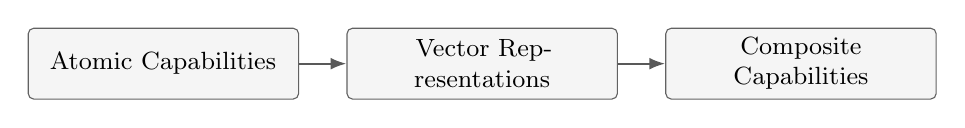
\begin{tikzpicture}[
  node distance=6mm,
  block/.style={draw=blue!65,fill=paleBlue,rounded corners=2pt,minimum height=9mm,
                text width=32mm,align=center,font=\small},
  arr/.style={-{Latex[length=2mm]},thick,color=muted}
]
\node[block] (atomic) {Atomic Capabilities};
\node[block,right=of atomic] (vecrep) {Vector Representations};
\node[block,right=of vecrep] (composite) {Composite Capabilities};
\draw[arr] (atomic)--(vecrep);
\draw[arr] (vecrep)--(composite);
\end{tikzpicture}
\end{center}

More broadly, this assignment is one step toward an architecture in which formally
specified applications are embedded, composed, and ultimately planned into executable
systems:

\begin{center}
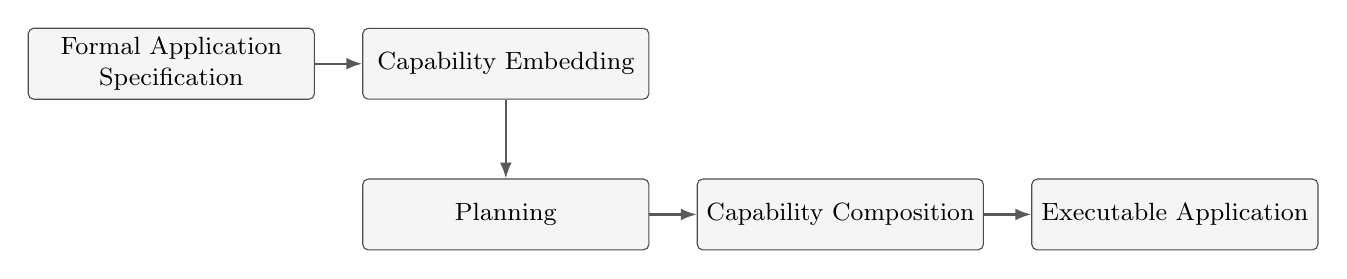
\begin{tikzpicture}[
  node distance=6mm,
  block/.style={draw=gold,fill=paleGold,rounded corners=2pt,minimum height=9mm,
                text width=34mm,align=center,font=\small},
  arr/.style={-{Latex[length=2mm]},thick,color=muted}
]
\node[block] (spec) {Formal Application\\Specification};
\node[block,right=of spec] (embed) {Capability Embedding};
\node[block,below=10mm of embed] (comp) {Planning};
\node[block,right=of comp] (plan) {Capability Composition};
\node[block,right=of plan] (exec) {Executable Application};
\draw[arr] (spec)--(embed);
\draw[arr] (embed)--(comp);
\draw[arr] (comp)--(plan);
\draw[arr] (plan)--(exec);
\end{tikzpicture}
\end{center}

The primary research question of this assignment is therefore:

\begin{keybox}[title={Primary research question}]
\large
How can formally specified states, goals, and executable capabilities be represented in a
vector space such that the representation preserves the relationships required for
capability compatibility, composition, and the construction of complex application
functionality?
\end{keybox}

\end{document}